% LaTeX source for ``การเรียนรู้ของเครื่องสำหรับเคมีควอนตัม (Machine Learning for Quantum Chemistry)''
% Copyright (c) 2022 รังสิมันต์ เกษแก้ว (Rangsiman Ketkaew).

% License: Creative Commons Attribution-NonCommercial-NoDerivatives 4.0 International (CC BY-NC-ND 4.0)
% https://creativecommons.org/licenses/by-nc-nd/4.0/

\chapter{การเรียนรู้ของเครื่อง}
\label{ch:ml}

%--------------------------
\section{ความสำคัญของ ML}
%--------------------------

การเรียนรู้ของเครื่องหรือ Machine Learning (ML) เป็นวิทยาการคอมพิวเตอร์ประเภทหนึ่งที่เราทำให้เครื่องจักรสมองกลเกิด \enquote{สติปัญญา} 
ซึ่งกระบวนการดังกล่าวนั้นเรียกว่าการเรียนรู้ของเครื่องจักร ซึ่งในบริบทนี้เครื่องจักรสมองกลที่เรารู้จักกันดีก็คือโปรแกรมที่ถูกติดตั้งอยู่ในคอมพิวเตอร์นั่นเอง
โดยวิธีการเรียนรู้ก็คือเราป้อนข้อมูลและคำตอบเข้าไปให้กับโปรแกรม โปรแกรมจะทำการสร้างโมเดลที่สามารถอธิบายความสัมพันธ์ระหว่างข้อมูลที่เราป้อนเข้าไปได้ 
ซึ่งขั้นตอนที่เกิดขึ้นระหว่างการเรียนรู้ก็คือการฝึกสอนโมเดล (Model Training) ซึ่งโปรแกรมสามารถแปลข้อมูลทั้งหมดเป็นโมเดลที่ปรับปรุงได้ 
นั่นหมายความว่าเทคโนโลยีการเรียนรู้ของเครื่องสามารถทำให้คอมพิวเตอร์เรียนรู้วิธีทำงานของมนุษย์โดยเฉพาะกิจกรรมที่ทำซ้ำหรือเกิดขึ้นแบบเดิมจนมีแบบแผน 
(Pattern) ที่สามารถเลียนแบบได้นั่นเอง 
\idxboth{การเรียนรู้ของเครื่อง}{Machine Learning}
\idxboth{การฝึกสอนโมเดล}{Model Training}

\begin{figure}[!htp]
    \centering
    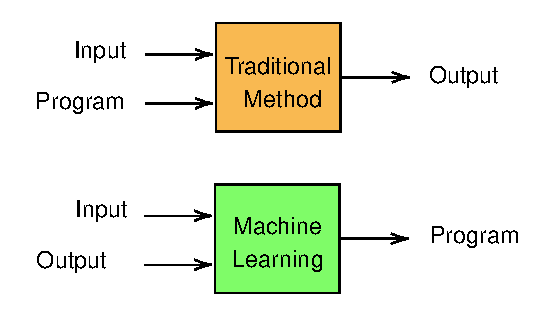
\includegraphics[scale=1]{fig/ch1-ML-concept.pdf}
    \caption{แผนภาพเปรียบเทียบการทำงานของโปรแกรมแบบดั้งเดิมกับการเรียนรู้ของเครื่อง}
    \label{fig:ml_paradigm}
\end{figure}

%--------------------------
\section{บทบาทของ ML ในควอนตัมเคมี}
%--------------------------

เคมีควอนตัม (Quantum Chemistry) เป็นแขนงหนึ่งของวิชาเคมีเชิงฟิสิกส์ (Physical Chemistry) ซึ่งเป็นการผสมผสานระหว่างกลศาสตร์ควอนตัม 
(Quantum Mechanics) กับการศึกษาอะตอมและโมเลกุลเข้าด้วยกัน กล่าวคือเรานำมาความทางด้านกลศาสตร์มาศึกษาอะตอมและโมเลกุล
โดยนักวิทยาศาสตร์ได้ศึกษาและค้นคว้างานวิจัยศาสตร์ด้านนี้มากว่าหนึ่งศควรรษ นับตั้งแต่ช่วงต้นปี ค.ศ. 1920 โดยได้มีการพัฒนาทฤษฎีต่าง ๆ มากมาย 
แต่สิ่งที่น่าสนใจก็คือจุดเปลี่ยนที่สำคัญของเคมีควอนตัมยุคใหม่ก็คือทฤษฎีความหนาแน่นเชิงฟังก์ชัน หรือ Density Functional Theory (DFT) 
ซึ่งถูกคิดค้นมากว่าครึ่งศตวรรษ ถ้าหากใครที่เคยเรียนวิชาเคมีเชิงฟิสิกส์หรือฟังการนำเสนอผลงานวิชาการตามงานประชุมวิชาการเคมีก็น่าจะเคยได้ยินชื่อทฤษฎีนี้กันมาบ้าง 
\idxboth{เคมีควอนตัม}{Quantum Chemistry}
\idxboth{ทฤษฎีความหนาแน่นเชิงฟังก์ชัน}{Density Functional Theory}

DFT เป็นทฤษฎีที่เรานำมาใช้ในการศึกษาคุณสมบัติของโมเลกุล ไม่ว่าจะเป็นขนาดเล็กอย่างเช่นโมเลกุลของสารประกอบอินทรีย์ และอนินทรีย์ 
หรือจะเป็นโมเลกุลขนาดใหญ่ เช่น โปรตีน, วัสดุโลหะ, และพอลิเมอร์ นั่นก็เพราะว่า DFT เป็นวิธีการคำนวณที่ให้ผลแม่นยำและใช้เวลาในการคำนวณที่ไม่นานมาก
นั่นจึงทำให้ทฤษฎี DFT ได้รับการเชิดชูเกียรติด้วยรางวัลโนเบลสาขาเคมีในปี ค.ศ. 1998 และถูกนำมาใช้อย่างแพร่หลายในงานวิจัยไม่เพียงแต่ในสาขาเคมีเท่านั้น 
แต่ยังรวมไปถึงสาขาฟิสิกส์และชีววิทยาอีกด้วย แต่ทว่าในความเป็นจริงนั้น DFT ไม่ได้ให้ผลการคำนวณที่แม่นยำสูงมากนักเมื่อเทียบกับวิธีฟังก์ชันคลื่นหรือ
Wavefunction Theory (WFT) และยังไม่สามารถคำนวณคุณสมบัติของระบบบางระบบได้ จึงทำให้ในปัจจุบันนั้นได้มีการพัฒนาระเบียบวิธีใหม่ ๆ 
ขึ้นมาเพื่อปรับปรุงประสิทธิภาพหรือความสามารถของ DFT ให้เทียบเท่ากับวิธีที่อ้างอิงด้วยวิธี

ในขณะเดียวกันนั้น ML ก็ถูกนำมาใช้ประโยชน์ในงานวิจัยเคมีมานานกว่า 30 ปีแล้ว แต่ในปัจจุบันนั้น เทคโนโลยีต่าง ๆ เช่น Supercomputing Cloud และ 
Graphical Processing Unit (GPU) ได้เข้ามามีบทบาทอย่างมากในวิทยาศาสตร์เชิงคำนวณ (Computaitonal Science) โดยเฉพาะเคมีเชิงคำนวณ 
(Computational Chemistry) จึงทำให้มีจุดเปลี่ยนที่ทำให้ความสนใจของนักวิจัยในช่วง 10 ปีที่ผ่านมานี้ในหันมาทำงานวิจัยโดยใช้ ML กันมากขึ้น 
นั่นก็เพราะว่าในปัจจุบันนั้น ML สามารถศึกษาได้ง่ายขึ้นเมื่อเทียบกับในอดีต ทุกวันนี้เราไม่จำเป็นต้องมานั่งเขียนโค้ดเพื่อสร้างโมเดล ML แบบเริ่มจากศูนย์กันแล้ว 
ตอนนี้เรามี Library แบบ Open-source ต่าง ๆ มากมายให้เลือกใช้ เช่น TensorFlow, PyTorch, Scikit-learn, หรือแม้แต่ Matlab 
ที่ก็มีฟังก์แบบสำเร็จรูปมาให้เราใช้งานได้เลย ซึ่งทำให้เราสามารถเลือกใช้โมเดล ML ต่าง ๆ ได้ตามต้องการ

ขอยกตัวอย่างงานวิจัยหนึ่งที่ตอนนี้กำลังเป็นหัวข้อที่มาแรง (อย่างน้อย ๆ ก็ ณ วันที่ผู้เขียนกำลังเขียนหนังสือเล่มนี้) นั่นคือการใช้ ML สร้างโมเดลที่ใช้ออกแบบ 
Exchange-Correlation (XC) Functional ที่สามารถนำไปใช้กับ DFT เพื่อศึกษาระบบได้หลายระบบ (Universal) ซึ่งถ้าหากเราทำสำเร็จหรือใกล้เคียง 
เราจะมีโมเดล XC ที่จะนำไปใช้ในการคำนวณอะไรก็ได้ เรียกได้ว่าเป็น XC สารพัดประโยชน์ (General-purpose) เลยก็ว่าได้ แต่ในความเป็นจริงนั้น 
XC นั้นก็เปรียบเสมือนเป็นกล่องดำ (Black Box) ซึ่งไม่มีใครที่รู้หน้าตาสมการหรือผลเฉลยทั่วไปของมันที่แน่นอน นั่นก็เพราะมันเป็นเทอมที่อธิบายอันตรกิริยาระหว่างอิเล็กตรอน 
ดังนั้นเราจึงทำได้เพียงหารูปแบบที่เป็นการประมาณเท่านั้น ตรงจุดนี้เองที่ ML ก็เข้ามามีบทบาทและทำให้งานวิจัยในช่วงระยะหลังนี้มีการพัฒนา ML เยอะมาก ๆ 
เพราะเป็นการประมาณค่าแบบหนึ่งที่ใช้หลักการทางสถิติเข้ามาช่วยในการหาความสัมพันธ์ระหว่างของสองสิ่งซึ่งให้ความแม่นยำสูงและไม่สิ้นเปลืองการคำนวณ 
ถึงแม้ว่าตอนนี้การนำ ML เข้ามาช่วยสำหรับการทำงานวิจัยทางด้านเคมึควอนตัม (และสาขาอื่น ๆ ด้วย) จะยังอยู่ในขั้นของการพัฒนา แต่สิ่งหนึ่งที่เราเห็นได้เลยก็คือ 
ML มันช่วยลดระยะเวลาในคำนวณคุณสมบัติเชิงอิเล็กทรอนิกส์ (Electronic Properties) ของโมเลกุลอย่างเห็นได้ชัด

\begin{table}[!htp]
    \centering
    \caption{ตารางเปรียบเทียบความซับซ้อนเชิงคำนวณของวิธีทางเคมีควอนตัม\cite{rupp2015} โดย $N$ คือจำนวนของอิเล็กตรอน}
    \label{tab:qm_complx}
    \small
    \begin{tabular}{lll}\toprule
    ตัวย่อ &วิธี &Runtime \\\midrule
    FCI &Full Configuration Interaction (CISDTQ) &$\mathcal{O}(N^{10})$ \\
    CC &Coupled Cluster (CCSD(T)) &$\mathcal{O}(N^{7})$ \\
    FCI &Full Configuration Interaction (CISD) &$\mathcal{O}(N^{6})$ \\
    MP2 &M$\o$llor-Plesset second order perturbation theory &$\mathcal{O}(N^{5})$ \\
    QMC &Quantum Monte Carlo &$\mathcal{O}(N^{3}) - \mathcal{O}(N^{4})$ \\
    HF &Hartree-Fock &$\mathcal{O}(N^{3}) - \mathcal{O}(N^{4})$ \\
    DFT &Density Functional Theory (Kohn-Sham) &$\mathcal{O}(N^{3})$ \\
    TB &Tight Binding &$\mathcal{O}(N^{3})$ \\
    MM &Molecular Mechanics &$\mathcal{O}(N^{2})$ \\
    \bottomrule
    \end{tabular}
\end{table}

ตารางที่ \ref{tab:qm_complx} แสดงค่าความซับซ้อนของการคำนวณของแต่ละวิธี โดยจะเห็นได้ว่าวิธี DFT นั้นมีความซับซ้อนคือ $\mathcal{O}(N^{3})$ 
นั่นคือมันเป็นสัดส่วนโดยตรงกับจำนวนของอิเล็กตรอนของระบบ ($N$) ยกกำลังสาม ซึ่งมาจากการที่เราจะต้องทำการ Diagonalize Hamiltonian 
ซึ่งความซับซ้อนของ Diagonalization สำหรับเมทริกซ์จตุรัสขนาด $n \times n$ คือ $\mathcal{O}(n^{3})$

\begin{adjustwidth}{-2.5 cm}{-2.5 cm}
    \centering
    \begin{threeparttable}[!htb]
    \caption{ตารางเปรียบเทียบความซับซ้อนเชิงคำนวณของวิธีทางเคมีควอนตัม\cite{zotero-328} โดย $n$ คือจำนวนของข้อมูล $p$ คือจำนวน Feature
    $n_{trees}$ คือจำนวนของต้นไม้ (Trees) $n_{sv}$ คือจำนวนของ Support Vectors $n_{L_{i}}$ คือจำนวนของ Neuron หรือ Node ของชั้นที่ $i$
    และ $t$ คือจำนวนของ Epochs ที่ใช้ในการเทรน Model}
    \label{tab:ml_complx}
    \small
    \begin{tabular}{lll}\toprule
    \multirow{2}{*}{อัลกอริทึม} &\multicolumn{2}{c}{Runtime} \\\cmidrule{2-3}
    &การเทรน Model &การทำนาย Output \\\midrule
    Decision Tree &$\mathcal{O}(n^{2}p)$ &$\mathcal{O}(p)$ \\
    Random Forest &$\mathcal{O}(n^{2}pn_{trees})$ &$\mathcal{O}(pn_{trees})$ \\
    Gradient Boosting (n\_{trees}) &$\mathcal{O}(npn_{trees})$ &$\mathcal{O}(pn_{trees})$ \\
    Linear Regression &$\mathcal{O}(p^{2}n+p^{3})$ &$\mathcal{O}(p)$ \\
    SVM (Kernel) &$\mathcal{O}(n^{2}p+n^{3})$ &$\mathcal{O}(n_{sv}p)$ \\
    Neural Network &$\mathcal{O}(npt*(n_{L_{1}}n_{L_{2}}+ n_{L_{2}}n_{L_{3}} + \dots)$ &$\mathcal{O}(pn_{L_{1}}+n_{L_{1}}n_{L_{2}}+ \dots)$ \\
    \bottomrule
    \end{tabular}
\end{threeparttable}
\end{adjustwidth}

ตารางที่ \ref{tab:ml_complx} แสดงค่าความซับซ้อนของการคำนวณของอัลกอริทึม ML แบบต่าง ๆ เช่นเดียวกับตารางก่อนหน้านี้ 
โดยอัลกอธิทึมที่แสดงนั้นถูกใช้กับโจทย์ปัญหา Classification และ Regression (ยกเว้น Linear Regression ที่ใช้สำหรับ Regression เท่านั้น)
จะเห็นได้ว่าความซับซ้อนของวิธี ML นั้นจะขึ้นอยู่กับจำนวนของข้อมูลและจำนวน Feature ของของข้อมูลแต่ละตัวเป็นหลัก ยกเว้นกรณีของการเรียนรู้เชิงลึก 
หรือ Neural Network (NN) เท่านั้นที่ความซับซ้อนของมันจะขึ้นอยู่กับจำนวนรอบที่ใช้ในการฝึกสอน (เทรน) Model และจำนวนชั้นของ Network

ถ้าหากเปรียบเทียบแล้วจะพบว่าวิธี ML นั้นมีความซับซ้อนน้อยกว่าวิธี QM อย่างมีนัยสำคัญ อย่างน้อย ๆ ก็ในระดับหลายเท่าตัว และยิ่งไปกว่านั้น
ความซับซ้อนเชิงการคำนวณในการทำนายค่า Output ของ Model ที่ผ่านการฝึกสอนมาแล้วนั้นต่ำมาก ซึ่งโดยส่วนใหญ่แล้วจะอยู่ในรูปของผลคูณเชิงเส้นแบบดีกรี 1 
ระหว่างจำนวนของข้อมูลกับจำนวนของ Feature นี่จึงเป็นเหตุผลที่ทำให้งานวิจัยทางด้านเคมี โดยเฉพาะด้าน QM ในช่วงระยะเวลา 10 ปีที่ผ่านมานั้น 
นักวิจัยเริ่มให้ความสนใจในการประยุกต์ใช้ ML เพื่อมาใช้ในการสร้าง Model สำหรับประมาณค่าหรือทำนายค่าต่าง ๆ ทางควอนตัม นั่นก็เพราะ ML เป็นวิธีที่สิ้นเปลืองน้อยกว่า

%--------------------------
\section{เริ่มต้นศึกษา ML}
%--------------------------

การมีความรู้พื้นฐานก่อนเริ่มศึกษา ML อย่างจริงจังนั้นมันเป็นสิ่งสำคัญ ผู้เขียนได้สรุป 5 สิ่งสำคัญที่ควรจะต้องรู้ 

\begin{enumerate}
    \item \textbf{พีชคณิตเชิงเส้นและแคลคูลัสแบบหลายตัวแปร} : ทั้งสองวิชานี้ถือว่าเป็นรากฐานของ ML เลยก็ว่าได้ 
    เพราะว่าโมเดลทุกรูปแบบของ ML นั้นต่างก็ล้วนแต่เป็นคณิตศาสตร์ ถ้าหากเราต้องการที่จะพัฒนาอังกอริธึมใหม่ ๆ 
    หรือปรับปรุงอัลกอริทึมที่มีอยู่แล้ว เราจะต้องอาศัยความรู้พีชคณิตเชิงเส้น (เวกเตอร์และเมทริกซ์) และแคลคูลัส (การหาอนุพันธ์) 
    แต่ถ้าหากว่าเราเน้นไปทางสายแอพพลิเคชัน เราก็อาจจะไม่จำเป็นต้องรู้แบบลึกหรือละเอียดมากก็ได้ เพราะว่าปัจจุบันนี้มี Library สำเร็จรูปให้เราเลือกใช้มากมาย
    \item \textbf{สถิติ} : เนื่องจากว่าในขั้นตอนก่อนที่จะเริ่มสร้างและเทรนโมเดล ML นั้น เราจะต้องใช้เวลาส่วนใหญ่ 
    (อาจจะมากถึง 80\%) ไปกับการรวบรวมข้อมูล ทำความสะอาดข้อมูล การศึกษาการกระจายตัวของข้อมูล การตั้งและทดสอบสมมติฐาน 
    การทำการถดถอย (Regression) การแยกประเภท (Classification) เราจึงจำเป็นจะต้องใช้สถิติเข้ามาช่วยเพื่อให้เข้าใจถึงรายละเอียด
    ของชุดข้อมูลที่เรากำลังจะเล่นกับมัน ยิ่งเข้าใจข้อมูลมากเท่าไหร่ ยิ่งช่วยให้เราสามารถเลือกใช้โมเดล ML ได้เหมาะสมเท่านั้น 
    \item \textbf{โปรแกรมมิ่ง} : สิ่งสำคัญลำดับถัดมาคือทักษะในการเขียนโปรแกรมหรือเขียนโค้ด ถึงแม้ว่าเราจะมีความรู้ด้านทฤษฎีที่แม่นยำ 
    แต่ถ้าหากเราไม่สามารถเขียนโปรแกรมได้ แล้วก็ไม่สามารถสร้างโมเดลหรือนำ ML มาใช้งานจริงได้เลย ดังนั้นเราควรจะต้องเรียนรู้การเขียนโปรแกรม
    ให้ได้อย่างน้อยสัก 1 ภาษา ซึ่งภาษาที่ได้รับความนิยมมากที่สุดสำหรับงานทางด้านวิทยาศาสตร์ข้อมูล ณ ตอนนี้คือภาษา Python 
    นั่นก็เพราะตัวภาษาเองมี Syntax ที่ง่าย มี Library ให้เลือกใช้เยอะ มี Community ที่ใหญ่มาก ไม่ต้องกลัวเลยว่าถ้าหากมีปัญหา
    เกี่ยวกับการเขียน Python แล้วจะไม่มีคนช่วยหรือหาวิธีแก้ปัญหาไม่ได้
    \item \textbf{แนวคิดของ ML} : แนวคิดหรือ Concept ทางด้าน ML (วิทยาศาสตร์ข้อมูล) เป็นสิ่งที่สำคัญมากเช่นเดียวกัน
    เราควรจะทราบคำศัพท์เฉพาะทางและความหมาย (Terminology) ประเภทของ ML แนวทางการนำ ML มาใช้ (Best Practice)
    \item \textbf{ฝึกทำโจทย์จริง} : ตัวช่วยที่ดีที่สุดให้เราเรียนรู้ ML ได้ง่ายและเร็วนั่นก็คือการฝึกฝน ลองหาโจทย์จริง ๆ มาฝึกทำ
    หรืออาจจะลองเก็บเกี่ยวประสบการณ์โดยเข้าร่วมการแข่งขันวิทยาศาสตร์ข้อมูล ซึ่ง ณ ปัจจุบันก็มีการจัดแข่งขันบ่อยมาก ๆ เรียกได้ว่ามีสนาม
    ให้ได้ฝึกฝนวิทยายุทธเป็นร้อย ๆ พัน ๆ เลย
\end{enumerate}

%--------------------------
\section{คำศัพท์ ML}
%--------------------------

\begin{description}[style=nextline]
    \item[Algorithm] วิธีหรือขั้นตอนกระบวนการคิดคำนวณทางคณิตศาสตร์เพื่อให้ได้ผลลัพธ์ออกมา
    \idxboth{อัลกอริทึม}{Algorithm}
    \item[Classification] การจำแนกข้อมูลหรือการทำนายค่าที่มีความไม่ต่อเนื่อง เช่น ประเภทของยานพาหนะ ชนิดของผลไม้
    \idxboth{การจำแนก}{Classification}
    \item[Data set หรือ Dataset] ชุดข้อมูลที่ได้เตรียมไว้ ประกอบไปด้วยข้อมูล Input และ/หรือ Output
    \idxboth{ชุดข้อมูล}{Data set}
    \item[Descriptor] Vector ของข้อมูล เช่น Feature vector
    \idxen{Descriptor}
    \item[Feature / Attribute] คุณลักษณะเด่นของข้อมูล
    \idxboth{คุณลักษณะเด่น}{Feature}
    \item[Model]  ชุดคำสั่งหรือโปรแกรมที่ถูกสร้างขึ้นมาโดยมีความสามารถในการคำนวณ ประมวลผลและตัดสินใจ
    \idxboth{แบบจำลอง}{Model}
    \item[Target / Class / Label / Output] คำตอบหรือเป้าหมายที่ต้องการคำนวณ ประมาณค่า หรือทำนาย
    \idxen{Target}
    \idxen{Class}
    \idxen{Label}
    \idxen{Output}
    \item[Training] กระบวนการสร้างและฝึกสอน Model โดยใช้ Training set 
    \idxboth{การฝึกสอน}{Training}
    \item[Prediction] กระบวนการทำนายค่าของ Model โดยจะทำนายค่า Output ของข้อมูลใหม่ที่ถูกป้อนเข้าไป
    \idxboth{การทำนาย}{Prediction}
    \item[Regression]  การทำนายค่าที่มีความต่อเนื่อง เช่น ราคาสินค้า ปริมาณน้ำมัน
    \idxen{Regression}
    \item[Reinforment learning] การเรียนรู้แบบเสริมแรง 
    \idxboth{การเรียนรู้แบบเสริมแรง}{Reinforment learning}
    \item[Representation] Descriptor ของโมเลกุลในรูปแบบสัญลักษณ์ (Symbolic) เช่น SMILES, InChI, สูตรโมเลกุล
    \idxen{Representation}
    \item[Supervised learning] การเรียนรู้ของ Model แบบมีผู้สอน (Output)
    \idxboth{การเรียนรู้แบบมีผู้สอน}{Supervised Learning}
    \item[Test set] ชุดข้อมูลที่ใช้ทดสอบความถูกต้องและแม่นยำของ Model
    \idxboth{ชุดข้อมูลสำหรับการทดสอบ}{Test set}
    \item[Training set] ชุดข้อมูลที่นำมาใช้ในการสอนคอมพิวเตอร์เพื่อสร้าง Model
    \idxboth{ชุดข้อมูลสำหรับการฝึกสอน}{Training set}
    \item[Unsupervised learning] การเรียนรู้ของ Model แบบไม่มีผู้สอน (Output-free)
    ซึ่งยังสามารถแบ่งออกได้เป็นสองประเภทคือ 1. Binary classification กับ 2. Multi-class classification
    \idxboth{การเรียนรู้แบบมีไม่มีผู้สอน}{Unsupervised Learning}
    \item[Validation set] ชุดข้อมูลสำหรับประเมินประสิทธิภาพของ Model ก่อนที่จะนำไปทดสอบกับ Test set จริง 
    โดย data set ประเภทนี้มักจะถูกนำมาใช้ในการทำ Cross-validation
    \idxboth{ชุดข้อมูลสำหรับการประเมินผล}{Validation set}
\end{description}
